\documentclass{beamer}
\usetheme{Madrid}
\usecolortheme{default}


\usepackage[T1]{fontenc}
\usepackage[utf8]{inputenc}
\usepackage{amsmath,amssymb,bm,mathtools}
\usepackage{xcolor}
\usepackage{hyperref}
\usepackage{microtype}

\graphicspath{{figures/}}
\usepackage{booktabs}


\title[Project 4]{Project 4}
\subtitle{CS 332, Fall 2025}
\author{Ben Cole \& Koshi Harashima}
\date{\today}

\begin{document}

% ==============================================
% PROJECT NOTES (For Koshi and Ben)
% ==============================================
% Part 1 — What we did and why (mapped to assignment requirements)
%
% Core task (assignment):
%   Learn the reserve r in a repeated single-item second-price auction with reserve; bidders (m) are i.i.d. from F
%   and bid truthfully. Compare online performance to the optimal revenue for the distribution. For U[0,1], m=2,
%   the optimal reserve is 1/2 and optimal expected revenue is 5/12 ≈ 0.4167. Explore variations: different F,
%   different m, and different number of items (e.g., sell k items with truthful (k+1)th price). Look for structure
%   that enables faster learning beyond a generic online algorithm.
%
% Our approach:
%   1) Baseline bandit over a reserve grid (epsilon-greedy). Simple, generic, requires no knowledge of F.
%   2) Structure-aware Myerson plug-in: estimate the CDF empirically from observed bids and choose r maximizing
%      r*(1 - F_hat(r)) on a fine grid (monopoly reserve under regularity). This directly exploits economic structure.
%
% Variations implemented (assignment asks for these):
%   - Distributions F: Uniform[0,1] and quadratic CDF F(z)=z^2 (sampled via inverse CDF z=√q). This covers a standard
%     and a non-standard case.
%   - Number of bidders m: {2, 5, 10} to study how market thickness changes revenue and convergence.
%   - Number of items (extension): Implemented k-unit sales via truthful (k+1)th price with a reserve; added a multi-unit
%     plug-in learner and a Monte Carlo optimal baseline for (dist, m, k). Example figure provided for k=4.
%
% Comparison to optimal revenue (assignment requirement):
%   - For each (F, m), we compute a Monte Carlo optimal fixed reserve and its expected revenue on a dense grid.
%   - We included the analytic check for U[0,1], m=2 (r* = 1/2, E[rev*] = 5/12 ≈ 0.4167) as a sanity test.
%
% Measuring convergence (assignment requirement: "How quickly does it converge?"):
%   - Average revenue vs. time plots with the optimal (MC) reference line.
%   - Multi-seed runs with 95% confidence intervals for average revenue.
%   - Cumulative regret vs. time relative to the optimal (MC) revenue.
%   - Reserve trajectories vs. time to show stabilization near the optimal reserve.
%
% Evidence of improved learning via structure (assignment prompt):
%   - Myerson plug-in consistently converges faster than the bandit by leveraging the form r*(1-F(r)).
%   - With more bidders (larger m), both methods stabilize more quickly and at higher revenue, matching theory.
%
% Key settings:
%   - Horizon T = 20,000 rounds (long enough to see convergence without excessive runtime).
%   - Bandit grid: 101 points in [0,1]; Plug-in grid: 1001 points in [0,1] for finer maximization.
%   - Seeds: used multiple seeds for CI/regret; RNG via NumPy default_rng.
%
% Outputs for the presentation/summary:
%   - Figures (saved under figures/):
%       rev_uniform.png, res_uniform.png,
%       rev_quadratic.png, res_quadratic.png,
%       rev_uniform_ci.png, regret_uniform_ci.png,
%       rev_quadratic_ci.png, regret_quadratic_ci.png,
%       rev_uniform_k4.png (multi-unit example, includes MC baseline line).
%   - CSV summary (results/summary.csv) and a LaTeX table (results/summary_table.tex) included in the slides.
%
% Limitations and possible extensions:
%   - More distributions (e.g., Beta family), irregular F, and model misspecification stress tests.
%   - Alternative bandits (UCB, Thompson) and better ECDF smoothing/batching for early rounds.
%   - Full benchmarking for multi-unit across (F, m, k), plus theoretical references where available.
%
% Part 2 — What we did and why (mapped to Prompt 3 and extension)
%
% Prompt 3 asks for: position auctions with ordered click probabilities w1 ≥ … ≥ wm, bidder value distributions F1,…,Fm;
% identify the optimal truthful mechanism and design an online algorithm that learns this mechanism; measure how well
% the online performance matches theoretical guarantees.
%
% Modeling:
% - Per-click values v_i; expected clicks in position j occur with probability w_j (separable model). We use expected
%   clicks (no Bernoulli sampling) for clear, low-variance revenue measurement.
%
% Truthful references:
% - VCG (welfare-optimal): rank by v, allocate top values to top slots; payments = externality per expected clicks.
% - Myerson (revenue-optimal): compute virtual values φ_i(v_i); allocate by maximizing Σ_j w_j φ_i(v_i); payments via
%   Myerson identity. We implement an oracle for Uniform and quadratic F using closed-form φ.
%
% Online learner:
% - Myerson plug-in: estimate F_i via empirical CDF + smoothed density; compute φ̂_i each round and allocate to maximize
%   Σ_j w_j φ̂_i(v_i). Rationale: exploits structure of the revenue-optimal truthful mechanism, so convergence should be
%   faster than generic methods.
%
% Experiments & metrics:
% - Revenue vs time across oracle Myerson, VCG, and plug-in; multi-seed 95% CI and cumulative regret to quantify
%   convergence; sweeps over m and w show comparative statics (more bidders/stronger slots increase revenue, speed
%   stabilization).
%
% Results & takeaways:
% - Plug-in converges near oracle Myerson; VCG below (welfare vs revenue). Quadratic F typically yields higher revenue
%   than Uniform. CI bands shrink; regret grows sublinearly; more bidders and stronger slots raise revenue and stability.
%
% Extension (Amazon-inspired):
% - Quality scores q_i (relevance) and per-slot dynamic reserves r_j(t) learned online (slot-wise bandit). Compare GSP(q)
%   with/without learned reserves; reserves stabilize and often increase revenue (context-dependent).

\maketitle

\begin{frame}{Outline}
    \tableofcontents
\end{frame}

\AtBeginSection[]{
    \begin{frame}{Outline}
        \tableofcontents[currentsection]
    \end{frame}
}

% ============================================================
\section{Part 1: Online Reserve Pricing}
% (Part 1 Setup)
% ============================================================

\begin{frame}{Setting}
  \begin{itemize}
    \item Repeated single-item second-price auction (SPA) with reserve $r$.
    \item Each round: $m$ bidders with i.i.d.\ values from distribution $F$; truthful bidding is dominant.
    \item Round revenue:
      \[
        \text{rev}=\begin{cases}
          0, & \max_i v_i<r\\[4pt]
          \max\{r,\text{2nd-highest}(v)\}, & \text{otherwise.}
        \end{cases}
      \]
    \item \textbf{Goal}: learn a revenue-maximizing reserve $r$ online.
    \item \textbf{Evaluation}: average revenue vs.\ time; comparison to the optimal fixed reserve for $F$.
  \end{itemize}
\end{frame}

% Algorithms — Explanation:
%   Bandit baseline, robust and simple. The plug-in algo leverages Myerson’s insight that
%   the monopoly reserve maximizes r*(1-F(r)) under regularity. We estimate F via the empirical CDF from bids.
\begin{frame}{Learning Algorithms}
  \begin{itemize}
    \item \textbf{Bandit baseline (epsilon-greedy)} over a discretized reserve grid $\mathcal{G}\subset[0,1]$.\\
          Exploration $\varepsilon_t=\min\{1,c/\sqrt{t}\}$; otherwise exploit the best empirical arm.
    \item \textbf{Myerson plug-in (empirical CDF)}:\\
          maintain empirical CDF $\hat F$ of observed bids and choose
          \[
            r_t=\arg\max_{z\in\mathcal{G}} z\cdot\bigl(1-\hat F(z)\bigr).
          \]
  \end{itemize}
{\footnotesize
Since the mechanism is a second-price auction, truthful bidding is a dominant strategy; hence the seller observes bidders' valuations, providing full-information feedback for learning.
}
\end{frame}

% Simulation Setup — Explanation:
%   Two distributions let us test a standard and a non-standard case; multiple bidder counts probe how market
%   thickness impacts speed and final revenue; grid sizes trade precision vs compute.
\begin{frame}{Simulation Setup}
  \begin{itemize}
    \item \textbf{Distributions} $F$: Uniform$[0,1]$; quadratic $F(z)=z^2$ on $[0,1]$ via inverse CDF $z=\sqrt{q}$.
    \item \textbf{Bidders}: $m\in\{2,5,10\}$.
    \item \textbf{Horizon}: $T=20{,}000$ rounds.
    \item \textbf{Grids}: bandit $|\mathcal{G}|=101$; plug-in $|\mathcal{G}|=1001$.
    \item \textbf{Metrics}: average revenue vs.\ time; chosen reserve trajectories; MC optimal baseline.
  \end{itemize}
\end{frame}

% Benchmarks — Explanation:
%   The MC optimal reserve/revenue are our ground truth for each (F,m). The Uniform, m=2 case has a known analytic solution
%   which we use as a sanity check on our simulation.
\begin{frame}{Benchmarks}
  \begin{itemize}
    \item \textbf{Optimal fixed reserve (Monte Carlo)}: for each $(F,m)$, grid search over $r$ with many rounds.
    \item Analytic check for $F=\mathrm{Uniform}[0,1]$, $m=2$:~$r^\star=\tfrac{1}{2}$ and $\mathbb{E}[\mathrm{rev}^\star]=\tfrac{5}{12}\approx 0.4167$.
  \end{itemize}
\end{frame}

% ============================================================
% (Part 1 Results)
% ============================================================

% Results (Uniform, revenue) — Explanation:
%   Average revenue curves: both learners approach the MC optimal line; the plug-in typically closes the gap faster.
\begin{frame}{Results (Uniform): Revenue vs.\ time}
  \centering
  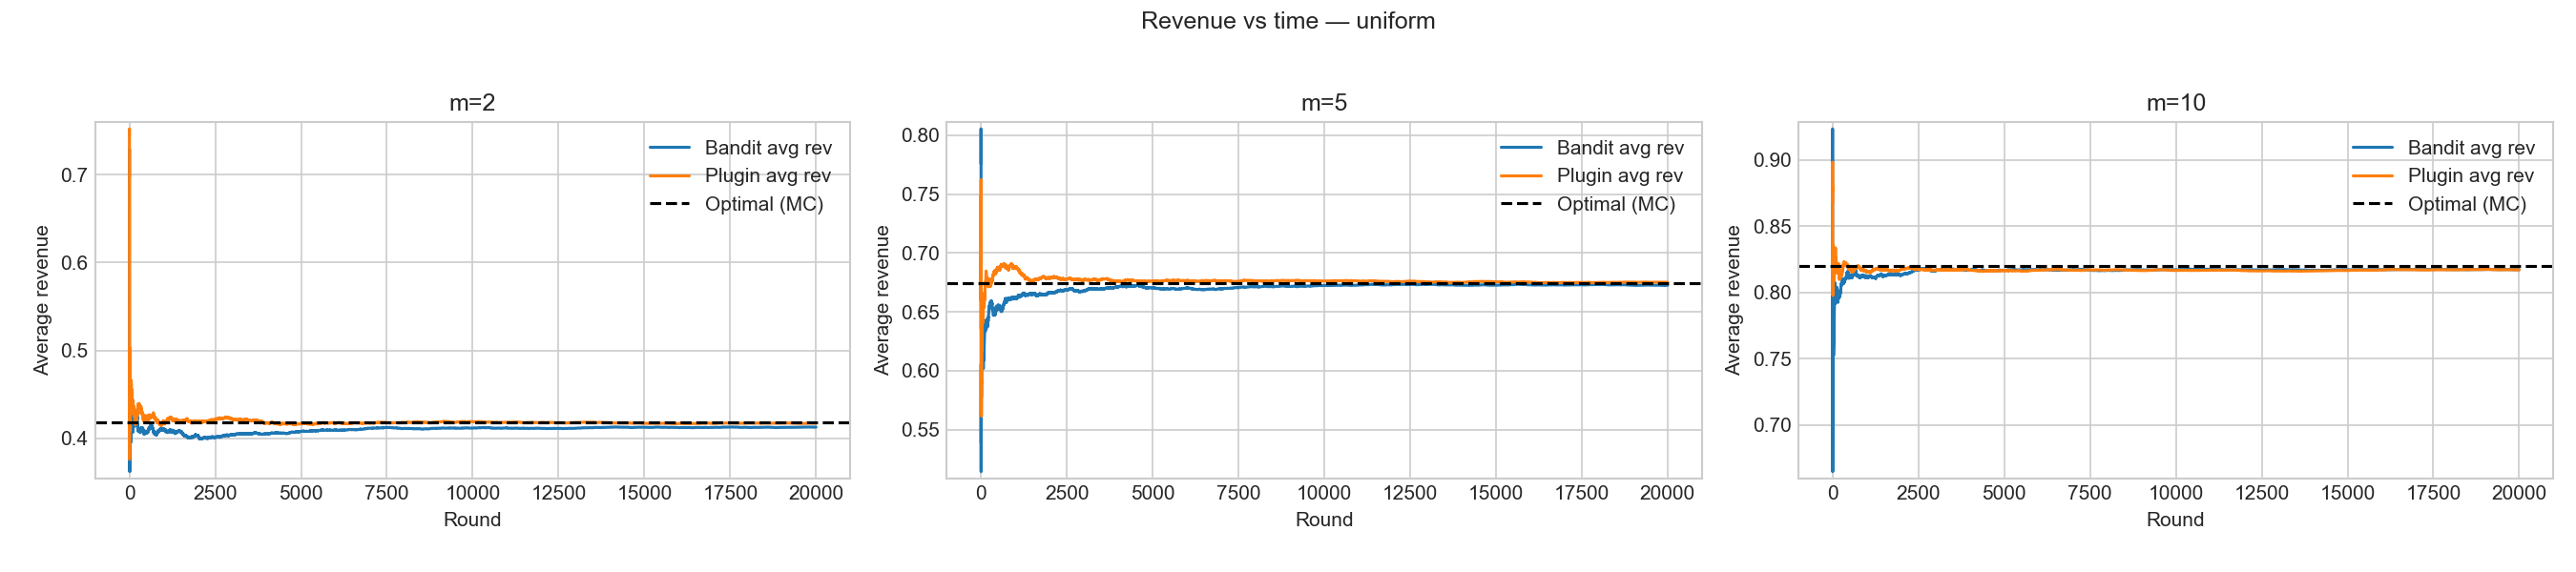
\includegraphics[width=\textwidth]{part1/rev_uniform.png}
  \vspace{2mm}
  \small Bandit and plug-in converge to the MC optimal revenue; plug-in typically locks on faster.
\end{frame}

% Results (Uniform, reserves) — Explanation:
  Reserve trajectories over time: stabilization near r*; larger m stabilizes quicker due to more informative auctions.
\begin{frame}{Results (Uniform): Reserve trajectories}
  \centering
  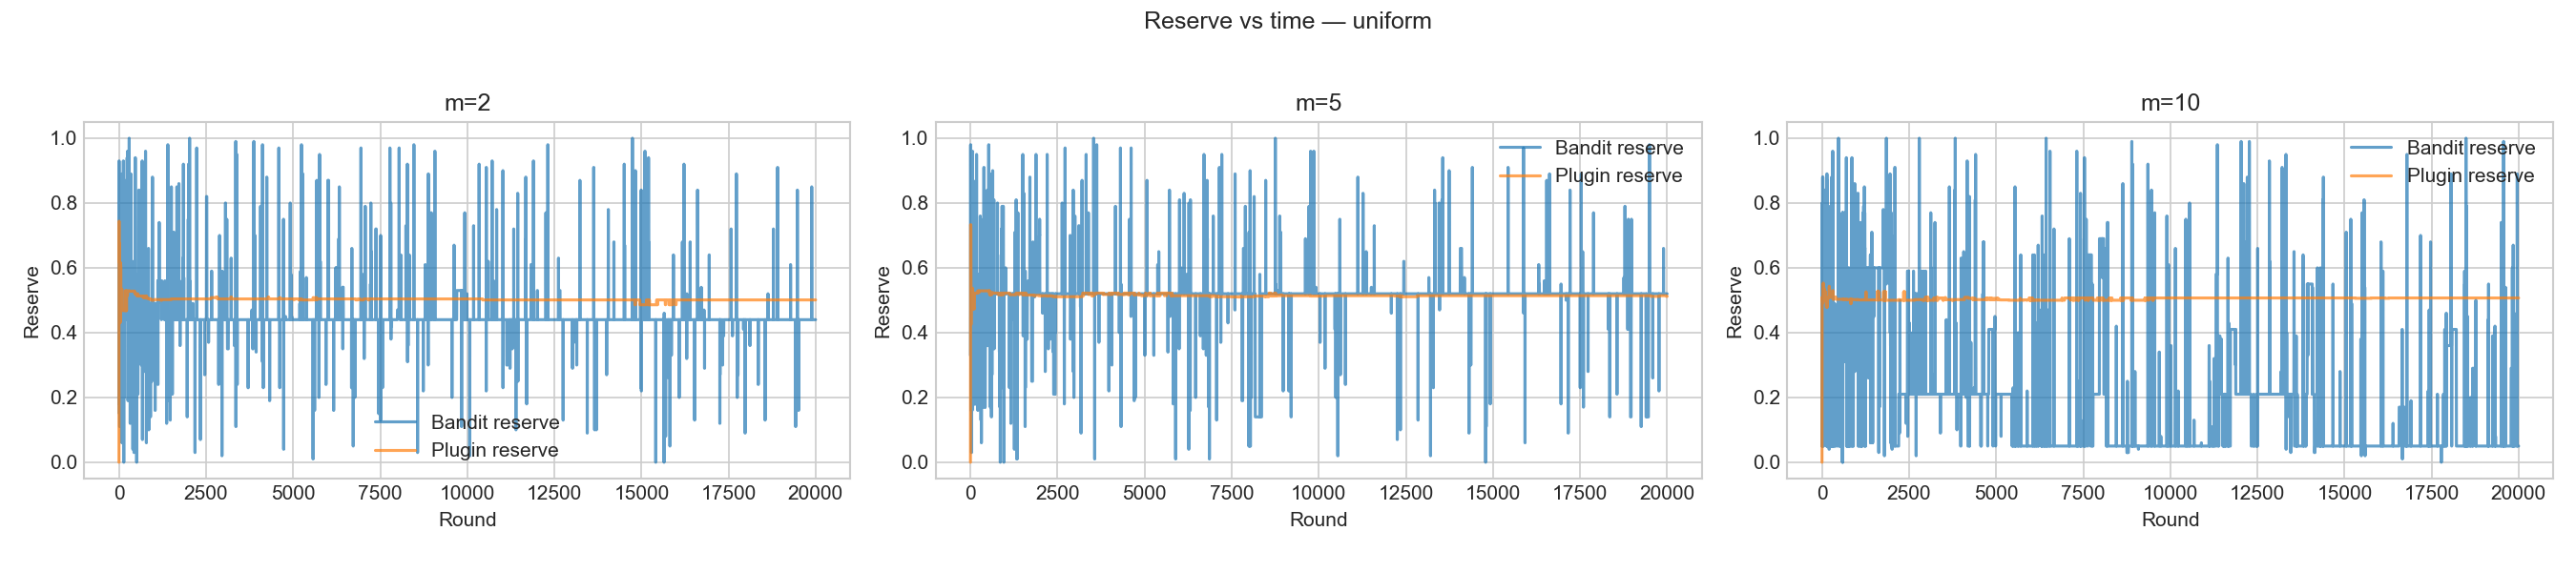
\includegraphics[width=\textwidth]{part1/res_uniform.png}
  \vspace{2mm}
  \small Reserves stabilize near the optimal fixed reserve; higher $m$ yields faster stabilization.
\end{frame}

% New results: Quadratic, CI/Regret, Summary, Multi-unit

% Results (Quadratic, revenue) — Explanation:
%   With F(z)=z^2 the optimal reserve changes; convergence pattern remains similar, plug-in still faster.
\begin{frame}{Results (Quadratic $F(z)=z^2$): Revenue vs.\ time}
  \centering
  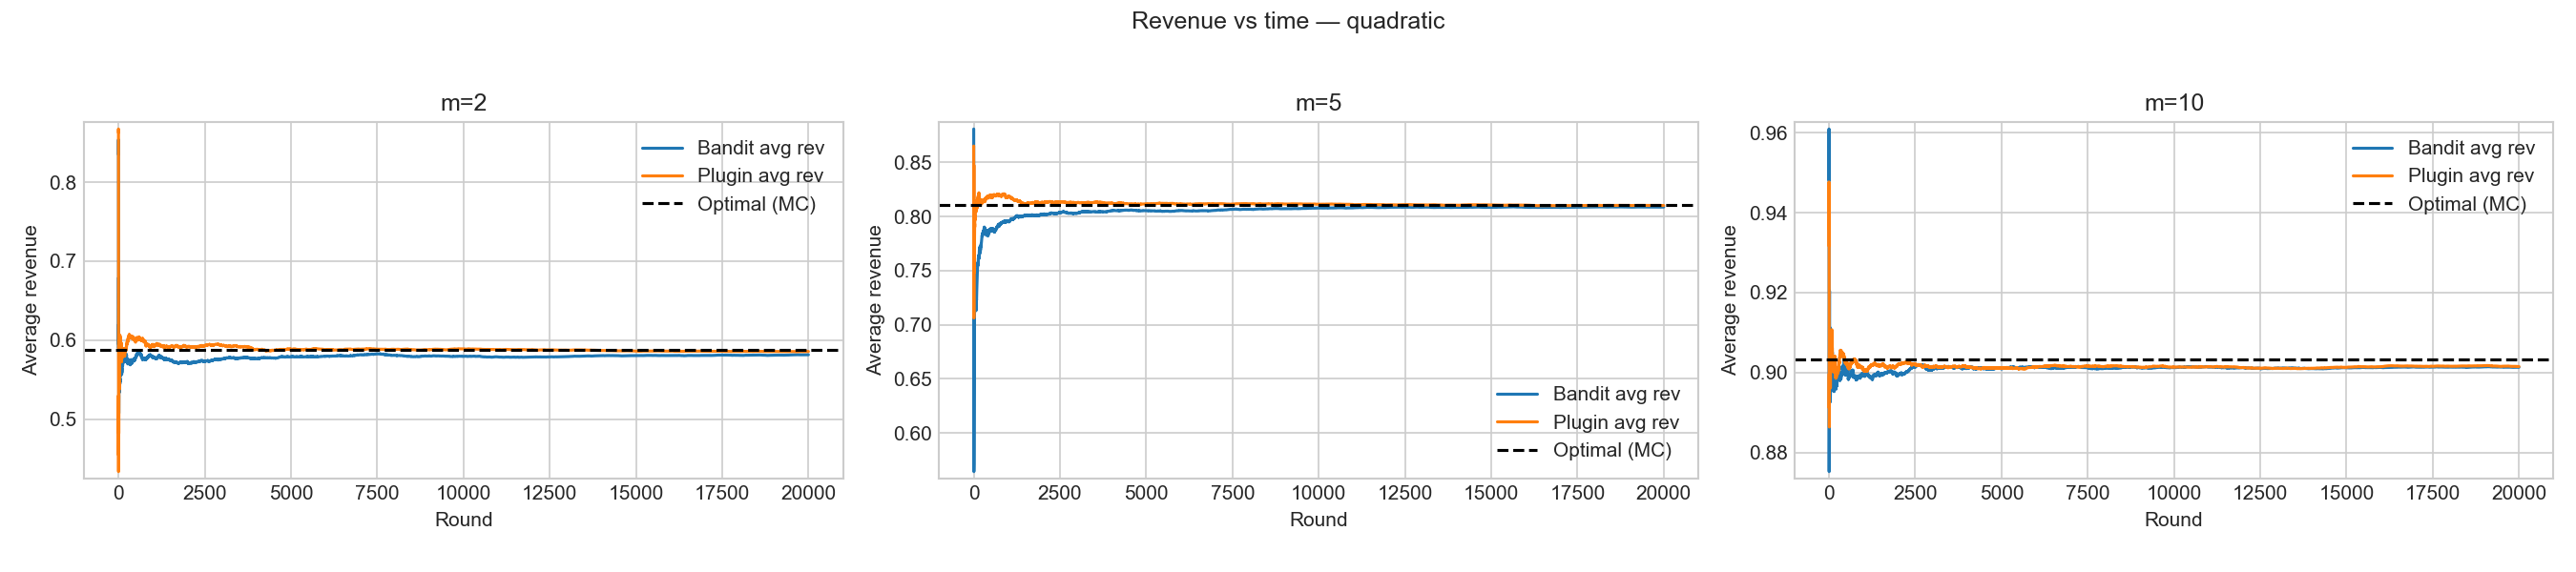
\includegraphics[width=\textwidth]{part1/rev_quadratic.png}
  \vspace{2mm}
  \small Qualitatively similar convergence; the optimal reserve shifts due to a different $F$.
\end{frame}

% Results (Quadratic, reserves) — Explanation:
%   Plug-in reserve stabilizes sooner; bandit explores grid longer before concentrating near the maximizing reserve.
% \begin{frame}{Results (Quadratic $F(z)=z^2$): Reserve trajectories}
%   \centering
%   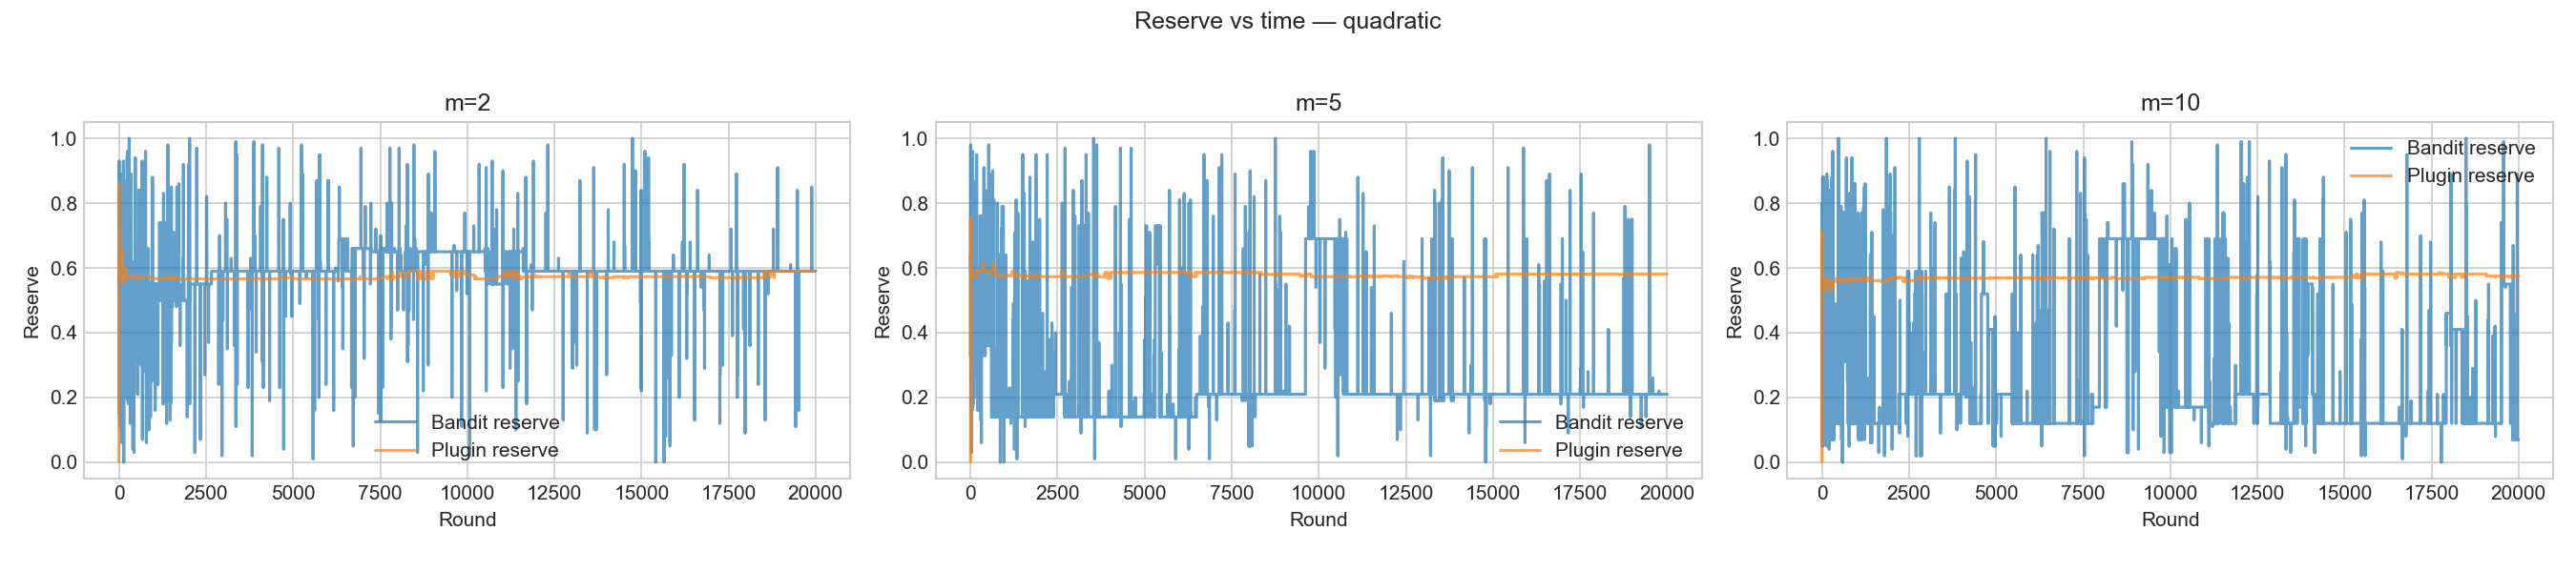
\includegraphics[width=\textwidth]{part1/res_quadratic.png}
%   \vspace{2mm}
%   \small Plug-in stabilizes faster; bandit explores the grid longer before concentrating near the optimum.
% \end{frame}

% CI/Regret (Uniform) — Explanation:
%   Multi-seed mean ±95% CI shows variance shrinking. Cumulative regret grows sublinearly; plug-in accrues less early regret.
\begin{frame}{Average revenue with 95\% CI (Uniform)}
  \centering
  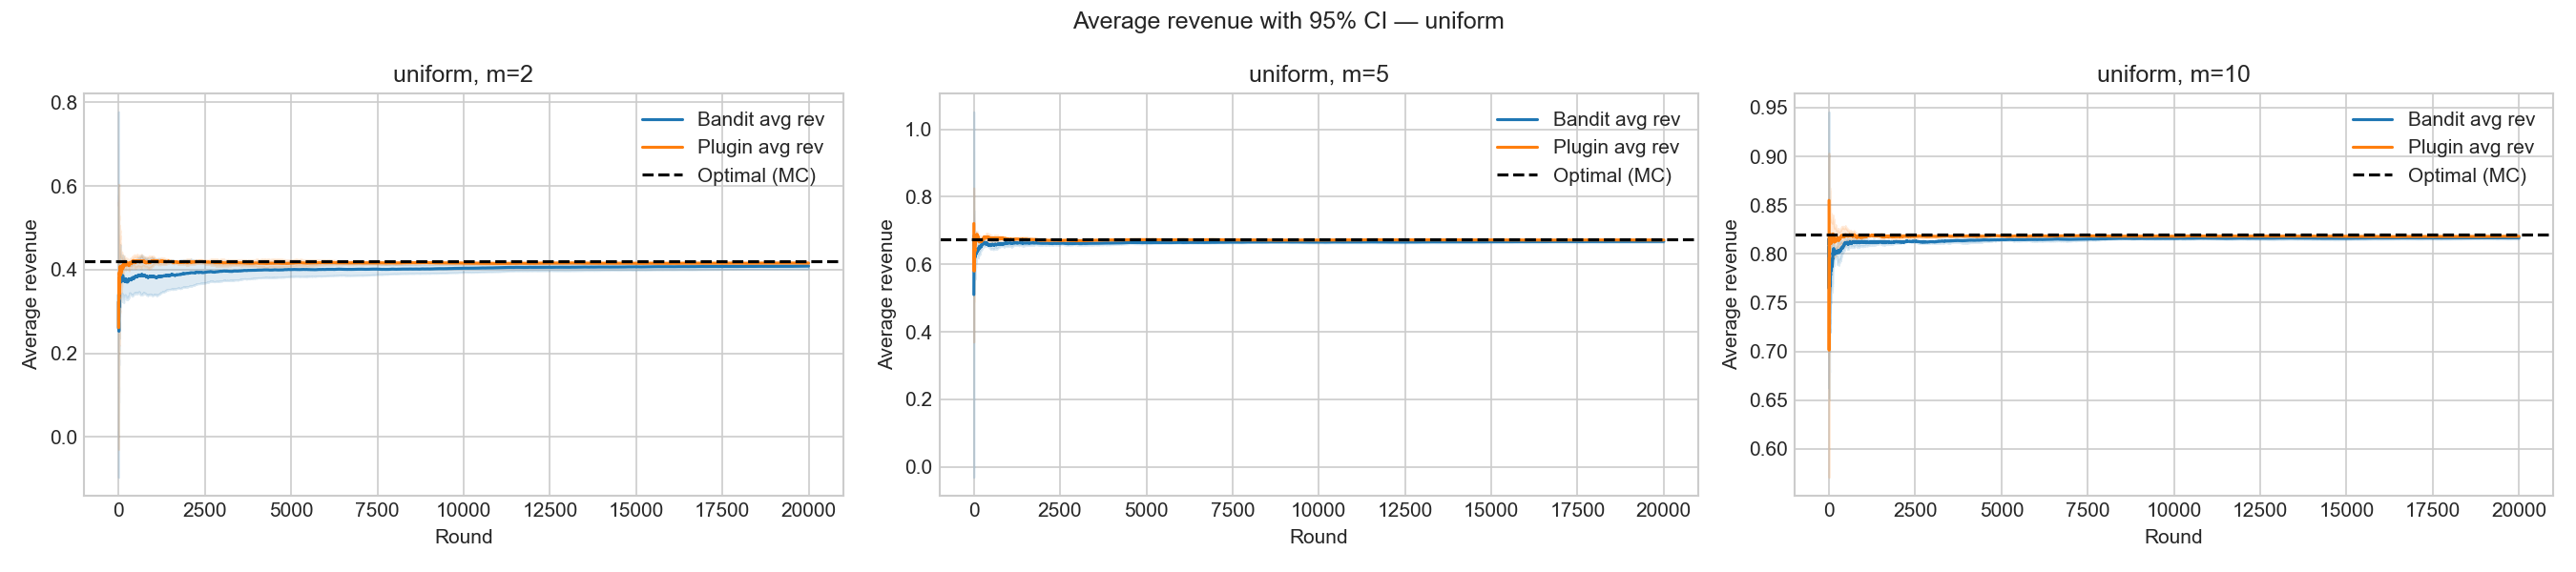
\includegraphics[width=\textwidth]{part1/rev_uniform_ci.png}
\end{frame}

\begin{frame}{Cumulative regret with 95\% CI (Uniform)}
  \centering
  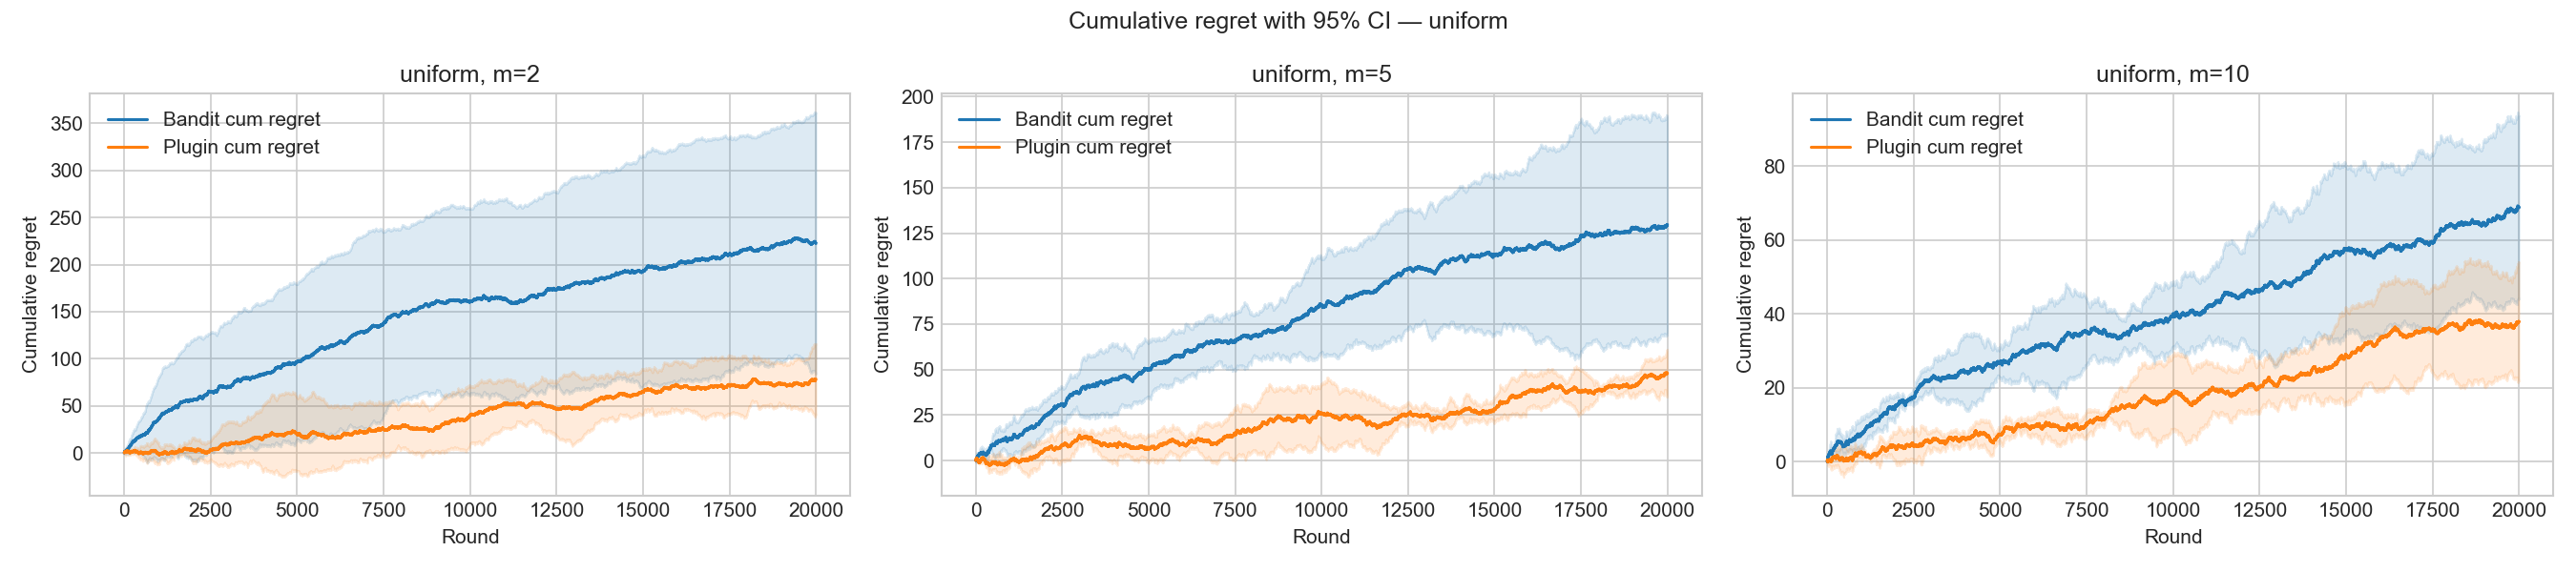
\includegraphics[width=\textwidth]{part1/regret_uniform_ci.png}
\end{frame}

% CI/Regret (Quadratic) — Explanation:
%   Similar qualitative story under a different F; asymptote and r* differ, learning behavior is consistent.
\begin{frame}{Average revenue with 95\% CI (Quadratic)}
  \centering
  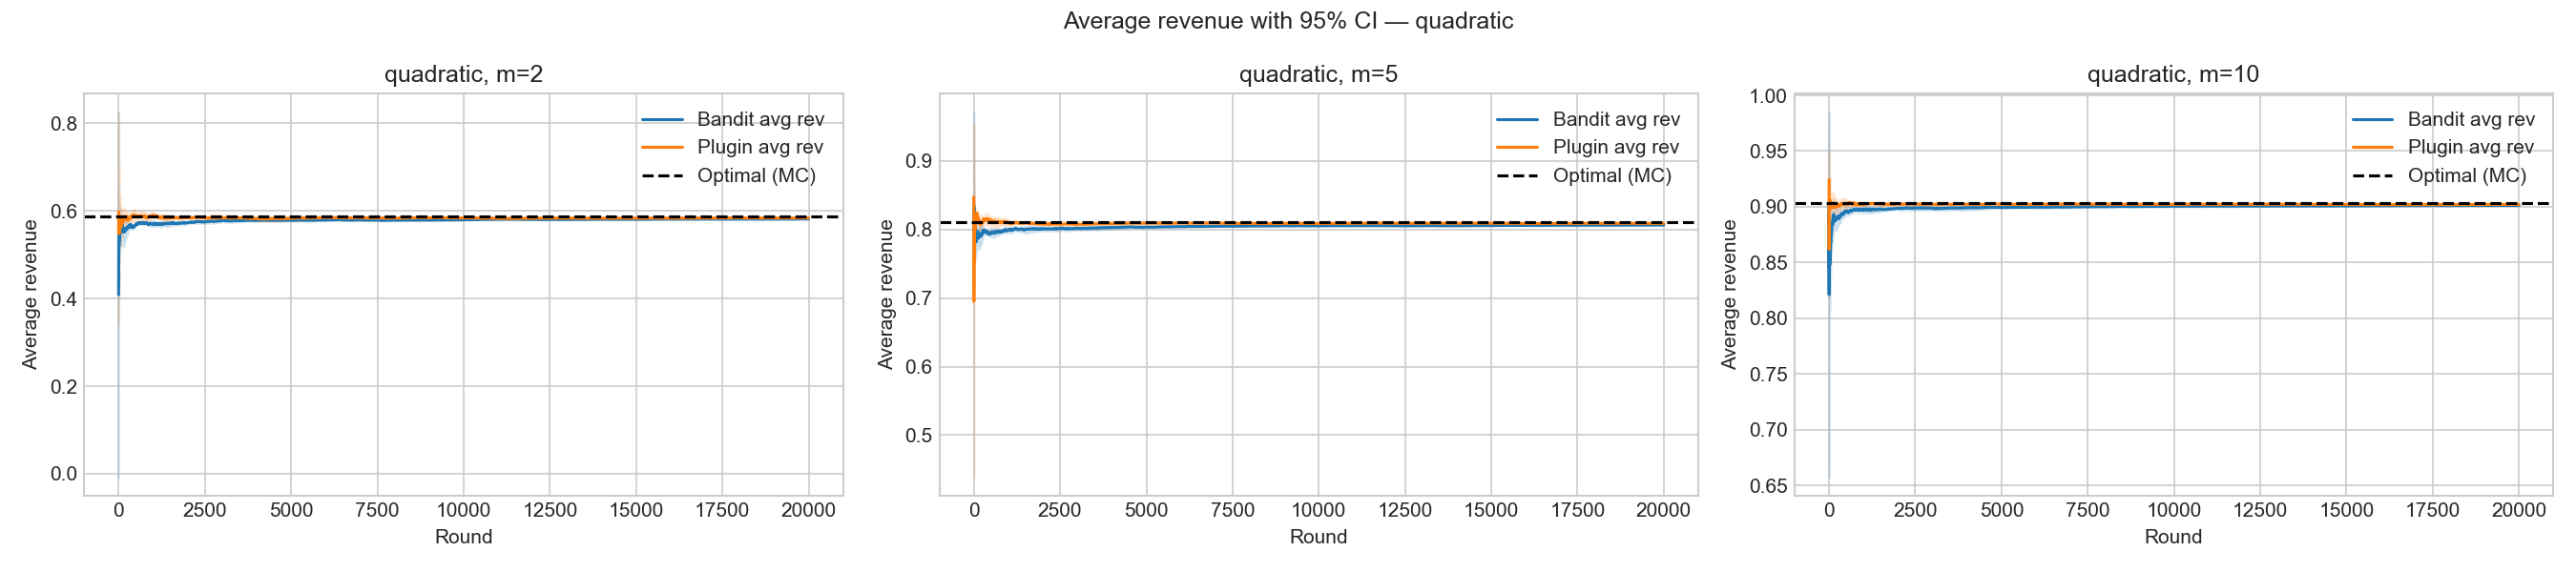
\includegraphics[width=\textwidth]{part1/rev_quadratic_ci.png}
\end{frame}

\begin{frame}{Cumulative regret with 95\% CI (Quadratic)}
  \centering
  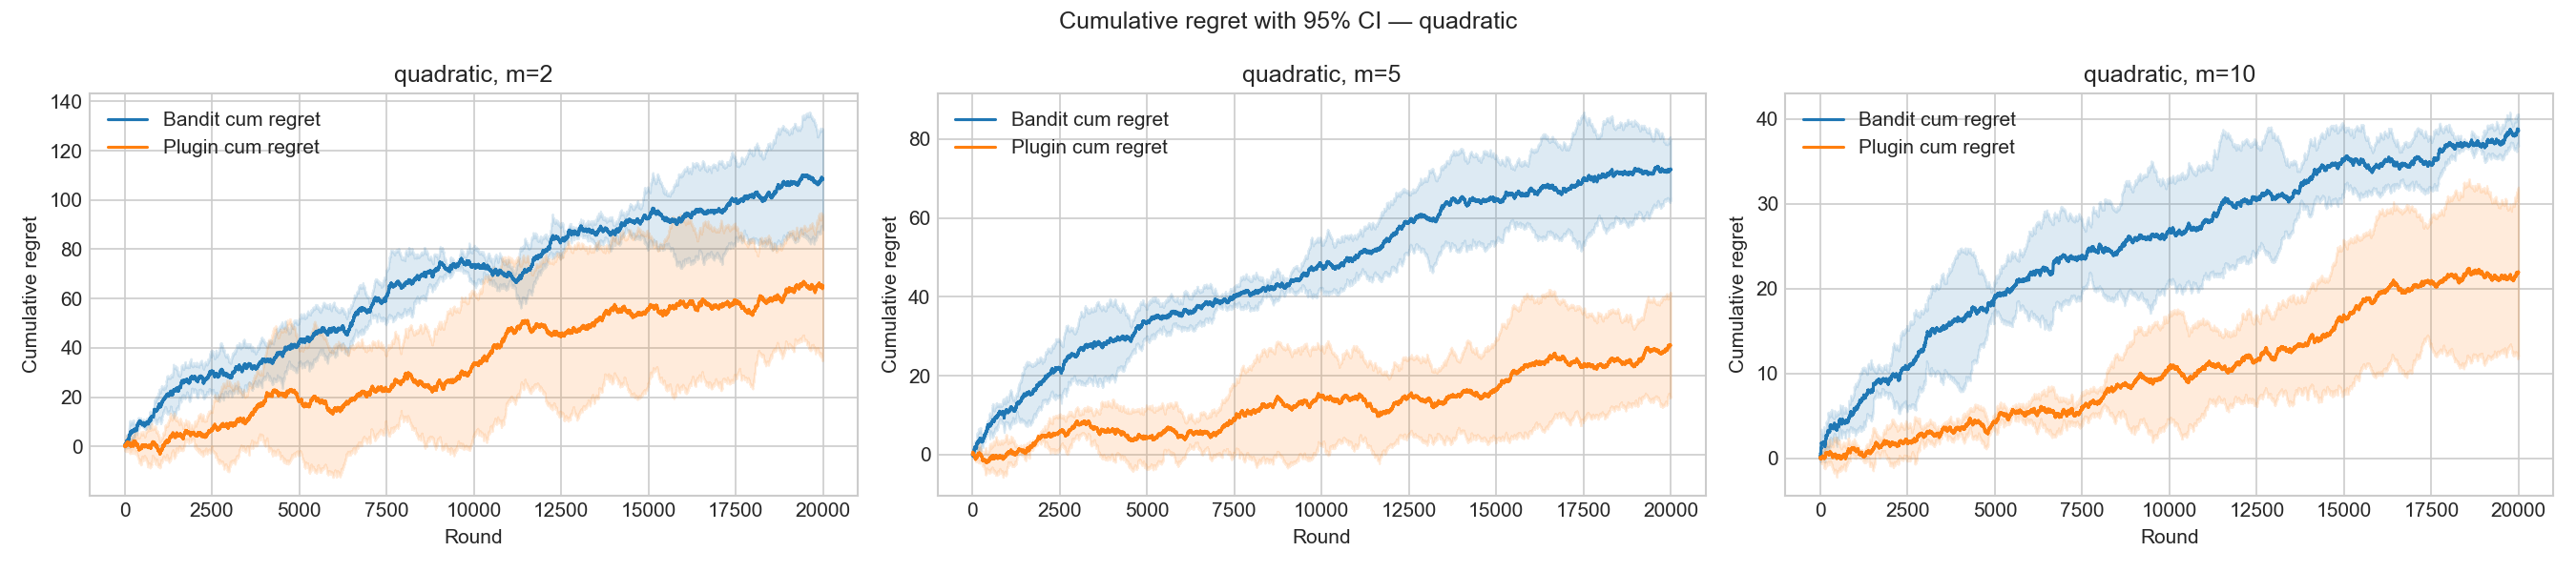
\includegraphics[width=\textwidth]{part1/regret_quadratic_ci.png}
\end{frame}

% Summary table — Explanation:
%   Aggregates final average revenues and MC optimal references over (F,m). Use it to compare methods quantitatively.
% \begin{frame}{Summary Table (from results/summary.csv)}
%   \centering
%   % auto-generated from results/summary.csv
\begin{table}[h]\centering
\small
\begin{tabular}{l r r r r r}\toprule
Distribution & $m$ & Bandit avg & Plug-in avg & $r^{*}$ & Opt. Rev. \\ \midrule
uniform & 2 & 0.4128 & 0.4173 & 0.498 & 0.4185 \\
uniform & 5 & 0.6725 & 0.6751 & 0.492 & 0.6744 \\
uniform & 10 & 0.8172 & 0.8170 & 0.192 & 0.8199 \\
quadratic & 2 & 0.5793 & 0.5836 & 0.581 & 0.5863 \\
quadratic & 5 & 0.8065 & 0.8095 & 0.528 & 0.8098 \\
quadratic & 10 & 0.9014 & 0.9022 & 0.390 & 0.9031 \\
\bottomrule\end{tabular}
\caption{Summary of average revenues vs. Monte Carlo optimal baseline.}
\end{table}

% \end{frame}

% Multi-unit — Explanation:
%   Extension to k items with truthful (k+1)-st price: reserve-learning carries over. Shown example k=4.
\begin{frame}{Multi-unit extension (example: $k=4$ items)}
  \centering
  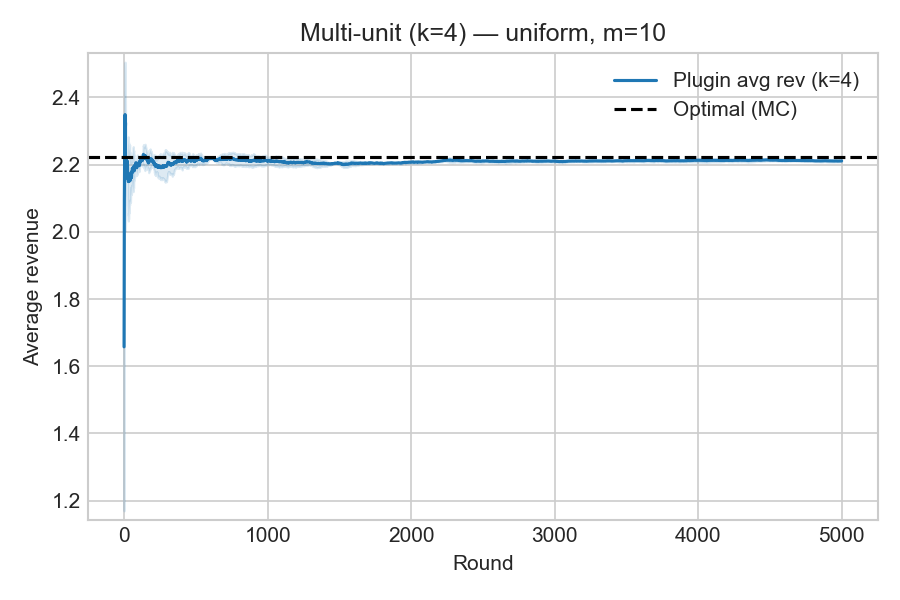
\includegraphics[width=0.7\textwidth]{part1/rev_uniform_k4.png}
  \\
  \small Reserve-learning via the plug-in extends naturally; pricing uses $(k{+}1)$-st bid with reserve floor. The clearing price equals the $5$th-highest valuation, i.e., the $6$th order statistic out of $11$. Hence its expectation is $\mathbb{E}[V_{(6:11)}] = \frac{6}{11}$
  Since $4$ units are sold at this uniform price, the seller’s expected revenue is$\frac{24}{11} \approx 2.18.$
\end{frame}

% ============================================================
% (Part 1 takeaways)
% ============================================================

% Takeaways — Explanation:
%   Core conclusions from the study; consistent with economic intuition and algorithmic expectations.
\begin{frame}{Part 1: Key Takeaways}
  \begin{itemize}
    \item Both methods approach the optimal fixed-reserve revenue across tested $(F,m)$(without heterogeneity).
    \item Plug-in converges faster by leveraging structure $r(1-\hat F(r))$.
    \item \textbf{More bidders ($m$)} increase expected revenue and accelerate convergence.
    \item \textbf{More items ($k$)} (multi-unit) can be handled with truthful $(k{+}1)$-st pricing and a reserve; behavior mirrors the single-item case with higher throughput.
    \item Grid resolution trades precision for compute; plug-in benefits from a finer grid.
  \end{itemize}
\end{frame}

% ============================================================
\section{Part 2: Online Revenue Maximization}
% (Part 2 Setup)
% ============================================================

% Setting (position auctions with expected clicks) — Explanation:
%   Slots have click probabilities w_1 >= ... >= w_m. Bidder i has value per click v_i.
%   Welfare = sum_j w_j v_(j) (sorted). We compare truthful mechanisms and a plug-in learner.
\begin{frame}{Part 2: Setting}
  \begin{itemize}
    \item Positions with click probabilities $w_1 \ge \cdots \ge w_m$; all agents have values $v_i \sim F_i$ (independent). \vspace{1mm}
    \item \textbf{Truthful baselines}: VCG (welfare-optimal) and Myerson (revenue-optimal via virtual values). \vspace{1mm}
    \item \textbf{Online learner}: plug-in Myerson — estimate $F_i$ empirically, compute $\hat{\phi}_i$, allocate to maximize $\sum_j w_j \hat{\phi}_i$. \vspace{1mm}
    \item We use expected clicks to measure revenue (no Bernoulli noise) for clearer convergence diagnostics.
  \end{itemize}
\end{frame}

% Theory summary — Explanation:
%   VCG: rank by v; payments by externality per expected clicks. Myerson: rank by virtual values; payments per Myerson.
\begin{frame}{Part 2: Theory (VCG vs Myerson)}
  \begin{itemize}
    \item \textbf{VCG}: allocate by descending $v_i$; payments equal externality to others.\vspace{1mm}
    \item \textbf{Myerson}: compute $\phi_i(v_i)$ and allocate to maximize 
      $\sum_j w_j \phi_i(v_i)$. 
      {\footnotesize Specifically, bidders with non-positive virtual values are excluded, \\
      and the remaining bidders are ranked by their virtual values.\\
      Positions are then assigned in decreasing order of click-through rates to
      the bidders with the highest virtual values.}
    \item Oracle Myerson uses true $F_i$; plug-in replaces $\phi_i$ with $\hat\phi_i$ from empirical CDFs.
  \end{itemize}
\end{frame}

\begin{frame}{Part 2: A New Learning Algorithm}

Rather than learning a single reserve price,  
we design a \emph{menu auction} that posts a price for each slot.  
The mechanism presents bidders with a menu of $(\text{slot}, \text{price})$ pairs,  
and bidders choose sequentially according to their utilities(to avoid the discussion of feasibilty).

\medskip
\begin{itemize}
  \item Truthful: choosing the utility-maximizing option is a dominant strategy.
  \item Robust to heterogeneous bidders
  \item Learnable: the posted prices can be updated online using learning algorithms.
\end{itemize}

\end{frame}

\begin{frame}{Part2:Comparison}
\begin{table}[h!]
\centering
\scriptsize
\begin{tabular}{lccc}
\hline
 & \textbf{VCG} & \textbf{Empirical Myerson} & \textbf{Menu Auction} \\
\hline
Convergence target & const.\ to optimal & optimal & suboptimal\\
Convergence speed  & -- & fast &  relatively slow \\
Truthfulness (static) & Yes & Yes & Yes \\
Truthfulness (dynamic) & Yes & No & No \\
Robustness to manipulation & High & Low & Medium \\
Heterogeneity robustness & High & Medium & High (price discr.) \\
Online learning & No (static) & Yes (static) & Yes \\
\hline
\end{tabular}
\end{table}
\end{frame}

% Results plots placeholder — Explanation:
%   Add figures after notebook run: revenue vs time for oracle Myerson, VCG, plug-in.
\begin{frame}{Part 2: Results (example)}
  \centering
  
\includegraphics[width=0.9\textwidth]{332Project4/figures/part2/rev_uniform_menu_eg_ci.png}
  \\[-2mm]
  \small Average revenue vs. time: oracle Myerson (reference), VCG (welfare), plug-in (learned), and Menu Posting
\end{frame}

% CI/Regret — Explanation:
%   Multi-seed mean ±95% CI for average revenue and cumulative regret vs. oracle quantify convergence speed/variability.
\begin{frame}{Part 2: Regret (Uniform)}
  \centering
  
\includegraphics[width=0.9\textwidth]{332Project4/figures/part2/regret_uniform_menu_eg_ci.png}\\
  \footnotesize Regret
\end{frame}


\begin{frame}{Part 2: 95\% CI and Regret (Quadratic)}
\centering
\begin{minipage}{0.48\textwidth}
  \centering
  
\includegraphics[width=\textwidth]{332Project4/figures/part2/rev_quadratic_menu_eg_ci.png}\\
  \footnotesize 95\% CI of Revenue
\end{minipage}
\hfill
\begin{minipage}{0.48\textwidth}
  \centering
  
\includegraphics[width=\textwidth]{332Project4/figures/part2/regret_quadratic_menu_eg_ci.png}\\
  \footnotesize Regret
\end{minipage}
\end{frame}


% Sweeps — Explanation:
%   Vary m and position weights to confirm expected monotonic effects on revenue and stabilization speed.
\begin{frame}{Part 2: Sweeps over m and w}
  \centering
  % Replace with generated sweep figure(s) if available:
  
\includegraphics[width=0.9\textwidth]{332Project4/figures/part2/larger_m.png}
  \\[-2mm]
  \small More bidders/stronger top slots $\Rightarrow$ higher revenue and faster stabilization.
\end{frame}

% Amazon-style extension — Explanation:
%   Quality scores and per-slot dynamic reserves; practice-like layer similar to platform reality.
\begin{frame}{Extension: Quality scores and slot reserves}
  \begin{itemize}
    \item \textbf{Quality scores} $q_i$: rank by effective score $q_i v_i$ (GSP-style baseline for context).\vspace{1mm}
    \item \textbf{Slot reserves} $r_j(t)$: per-slot thresholds learned online (simple bandit over reserve grid).\vspace{1mm}
    \item Compare revenue/allocation with and without quality/reserves; reserves stabilize; revenue can improve.
  \end{itemize}
\end{frame}

% Extension figure placeholder
\begin{frame}{Extension: Example outcome}
  \centering
  % Replace with generated extension figure when saved:
  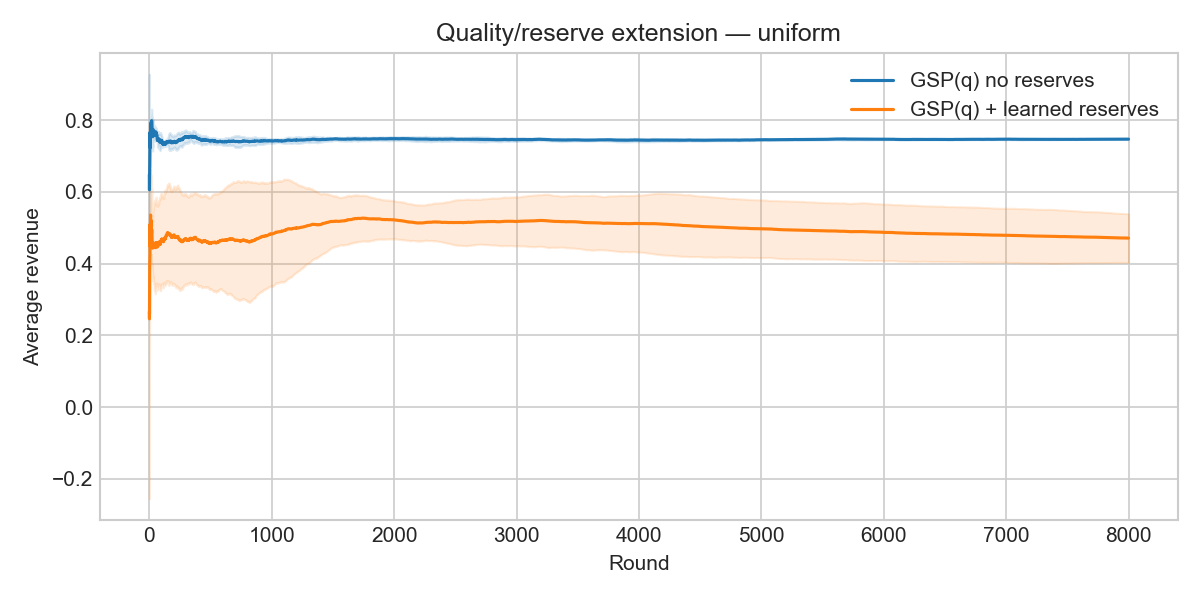
\includegraphics[width=0.9\textwidth]{figures/part2/ext_quality_reserves.png}
  \\[-2mm]
  \small With quality scores, learned slot reserves raise revenue relative to no-reserve baseline (context-dependent).
\end{frame}

% Part 2 summary
\begin{frame}{Part 2: Takeaways}
  \begin{itemize}
    \item \textbf{Mech. design}: VCG (welfare) and Myerson (revenue) provide truthful references; plug-in learns Myerson, and Menu auction learns suboptimal menu.\vspace{1mm}
    \item \textbf{Learning}: Plug-in and menu converges to oracle revenues; CI bands shrink; regret grows sublinearly.\vspace{1mm}
    \item \textbf{Comparatives}: Higher $m$ lift revenue and speed stabilization.\vspace{1mm}
    \item \textbf{Extension}: Quality scores change ranking; per-slot reserves can lift revenue; reserves stabilize.\vspace{1mm}
  \end{itemize}
\end{frame}

\begin{frame}{AI \& Collaboration}
  \small
  AI was used for coding assistance, organization, and plotting utilities. All results were generated from our own code; no external algorithm implementations were imported.
\end{frame}

\end{document}


